% Options for packages loaded elsewhere
% Options for packages loaded elsewhere
\PassOptionsToPackage{unicode}{hyperref}
\PassOptionsToPackage{hyphens}{url}
\PassOptionsToPackage{dvipsnames,svgnames,x11names}{xcolor}
%
\documentclass[
  letterpaper,
  DIV=11,
  numbers=noendperiod]{scrartcl}
\usepackage{xcolor}
\usepackage{amsmath,amssymb}
\setcounter{secnumdepth}{-\maxdimen} % remove section numbering
\usepackage{iftex}
\ifPDFTeX
  \usepackage[T1]{fontenc}
  \usepackage[utf8]{inputenc}
  \usepackage{textcomp} % provide euro and other symbols
\else % if luatex or xetex
  \usepackage{unicode-math} % this also loads fontspec
  \defaultfontfeatures{Scale=MatchLowercase}
  \defaultfontfeatures[\rmfamily]{Ligatures=TeX,Scale=1}
\fi
\usepackage{lmodern}
\ifPDFTeX\else
  % xetex/luatex font selection
\fi
% Use upquote if available, for straight quotes in verbatim environments
\IfFileExists{upquote.sty}{\usepackage{upquote}}{}
\IfFileExists{microtype.sty}{% use microtype if available
  \usepackage[]{microtype}
  \UseMicrotypeSet[protrusion]{basicmath} % disable protrusion for tt fonts
}{}
\makeatletter
\@ifundefined{KOMAClassName}{% if non-KOMA class
  \IfFileExists{parskip.sty}{%
    \usepackage{parskip}
  }{% else
    \setlength{\parindent}{0pt}
    \setlength{\parskip}{6pt plus 2pt minus 1pt}}
}{% if KOMA class
  \KOMAoptions{parskip=half}}
\makeatother
% Make \paragraph and \subparagraph free-standing
\makeatletter
\ifx\paragraph\undefined\else
  \let\oldparagraph\paragraph
  \renewcommand{\paragraph}{
    \@ifstar
      \xxxParagraphStar
      \xxxParagraphNoStar
  }
  \newcommand{\xxxParagraphStar}[1]{\oldparagraph*{#1}\mbox{}}
  \newcommand{\xxxParagraphNoStar}[1]{\oldparagraph{#1}\mbox{}}
\fi
\ifx\subparagraph\undefined\else
  \let\oldsubparagraph\subparagraph
  \renewcommand{\subparagraph}{
    \@ifstar
      \xxxSubParagraphStar
      \xxxSubParagraphNoStar
  }
  \newcommand{\xxxSubParagraphStar}[1]{\oldsubparagraph*{#1}\mbox{}}
  \newcommand{\xxxSubParagraphNoStar}[1]{\oldsubparagraph{#1}\mbox{}}
\fi
\makeatother


\usepackage{longtable,booktabs,array}
\usepackage{calc} % for calculating minipage widths
% Correct order of tables after \paragraph or \subparagraph
\usepackage{etoolbox}
\makeatletter
\patchcmd\longtable{\par}{\if@noskipsec\mbox{}\fi\par}{}{}
\makeatother
% Allow footnotes in longtable head/foot
\IfFileExists{footnotehyper.sty}{\usepackage{footnotehyper}}{\usepackage{footnote}}
\makesavenoteenv{longtable}
\usepackage{graphicx}
\makeatletter
\newsavebox\pandoc@box
\newcommand*\pandocbounded[1]{% scales image to fit in text height/width
  \sbox\pandoc@box{#1}%
  \Gscale@div\@tempa{\textheight}{\dimexpr\ht\pandoc@box+\dp\pandoc@box\relax}%
  \Gscale@div\@tempb{\linewidth}{\wd\pandoc@box}%
  \ifdim\@tempb\p@<\@tempa\p@\let\@tempa\@tempb\fi% select the smaller of both
  \ifdim\@tempa\p@<\p@\scalebox{\@tempa}{\usebox\pandoc@box}%
  \else\usebox{\pandoc@box}%
  \fi%
}
% Set default figure placement to htbp
\def\fps@figure{htbp}
\makeatother





\setlength{\emergencystretch}{3em} % prevent overfull lines

\providecommand{\tightlist}{%
  \setlength{\itemsep}{0pt}\setlength{\parskip}{0pt}}



 


\usepackage{booktabs}
\usepackage{longtable}
\usepackage{array}
\usepackage{multirow}
\usepackage{wrapfig}
\usepackage{float}
\usepackage{colortbl}
\usepackage{pdflscape}
\usepackage{tabu}
\usepackage{threeparttable}
\usepackage{threeparttablex}
\usepackage[normalem]{ulem}
\usepackage{makecell}
\usepackage{xcolor}
\KOMAoption{captions}{tableheading}
\makeatletter
\@ifpackageloaded{caption}{}{\usepackage{caption}}
\AtBeginDocument{%
\ifdefined\contentsname
  \renewcommand*\contentsname{Table of contents}
\else
  \newcommand\contentsname{Table of contents}
\fi
\ifdefined\listfigurename
  \renewcommand*\listfigurename{List of Figures}
\else
  \newcommand\listfigurename{List of Figures}
\fi
\ifdefined\listtablename
  \renewcommand*\listtablename{List of Tables}
\else
  \newcommand\listtablename{List of Tables}
\fi
\ifdefined\figurename
  \renewcommand*\figurename{Figure}
\else
  \newcommand\figurename{Figure}
\fi
\ifdefined\tablename
  \renewcommand*\tablename{Table}
\else
  \newcommand\tablename{Table}
\fi
}
\@ifpackageloaded{float}{}{\usepackage{float}}
\floatstyle{ruled}
\@ifundefined{c@chapter}{\newfloat{codelisting}{h}{lop}}{\newfloat{codelisting}{h}{lop}[chapter]}
\floatname{codelisting}{Listing}
\newcommand*\listoflistings{\listof{codelisting}{List of Listings}}
\makeatother
\makeatletter
\makeatother
\makeatletter
\@ifpackageloaded{caption}{}{\usepackage{caption}}
\@ifpackageloaded{subcaption}{}{\usepackage{subcaption}}
\makeatother
\usepackage{bookmark}
\IfFileExists{xurl.sty}{\usepackage{xurl}}{} % add URL line breaks if available
\urlstyle{same}
\hypersetup{
  pdftitle={Proyecto Inferencia II: Climbers},
  pdfauthor={Santiago Robatto, Diego Da Rosa, Sofía Terra, Nahuel Bizoso},
  colorlinks=true,
  linkcolor={blue},
  filecolor={Maroon},
  citecolor={Blue},
  urlcolor={Blue},
  pdfcreator={LaTeX via pandoc}}


\title{Proyecto Inferencia II: Climbers}
\author{Santiago Robatto, Diego Da Rosa, Sofía Terra, Nahuel Bizoso}
\date{}
\begin{document}
\maketitle


\begin{verbatim}
# A tibble: 2,076 x 24
   expedition_id member_id    peak_id peak_name   year season sex     age
   <chr>         <fct>        <fct>   <fct>      <dbl> <fct>  <fct> <dbl>
 1 AMAD81101     AMAD81101-03 AMAD    Ama Dablam  1981 Spring M        28
 2 AMAD81101     AMAD81101-04 AMAD    Ama Dablam  1981 Spring M        27
 3 AMAD81101     AMAD81101-02 AMAD    Ama Dablam  1981 Spring M        35
 4 AMAD81101     AMAD81101-05 AMAD    Ama Dablam  1981 Spring M        37
 5 AMAD81101     AMAD81101-06 AMAD    Ama Dablam  1981 Spring M        43
 6 AMAD81101     AMAD81101-07 AMAD    Ama Dablam  1981 Spring M        38
 7 AMAD81101     AMAD81101-08 AMAD    Ama Dablam  1981 Spring M        23
 8 AMAD81101     AMAD81101-01 AMAD    Ama Dablam  1981 Spring M        36
 9 AMAD81101     AMAD81101-09 AMAD    Ama Dablam  1981 Spring M        48
10 AMAD81101     AMAD81101-11 AMAD    Ama Dablam  1981 Spring M        25
# i 2,066 more rows
# i 16 more variables: citizenship <fct>, expedition_role <fct>, hired <lgl>,
#   highpoint_metres <dbl>, success <lgl>, solo <lgl>, oxygen_used <lgl>,
#   died <lgl>, death_cause <fct>, death_height_metres <dbl>, injured <lgl>,
#   injury_type <fct>, injury_height_metres <dbl>, count <int>,
#   height_metres <dbl>, first_ascent_year <dbl>
\end{verbatim}

\subsubsection{Introducción}\label{introducciuxf3n}

\begin{itemize}
\item
  El dataset contiene información de interacciones comerciales
  cliente--propiedad en el mercado inmobiliario y cuenta con 24
  variables y 2076 observaciones.
\item
  Algunas variables refieren a las características sociodemográficas del
  lead/cliente, mientras que otras describen los atributos del inmueble
  visitado.
\item
  La variable de interés es la decisión de compra (compra: 1 = compró el
  inmueble, 0 = no compró), la cual es binaria.
\item
  La compra representa un evento de conversión comercial real, análogo a
  un cierre de venta.
\item
  En el contexto original, el éxito se daba al alcanzar la cima del
  pico; en esta reconversión, el éxito se interpreta como que el cliente
  decidió adquirir la propiedad que visitó, lo cual nos lleva
  naturalmente a plantear un modelo de clasificación con enlace
  logístico para estimar probabilidades de conversión.
\item
  Esto nos hace pensar en un modelo logístico (regresión logística) para
  explicar y/o predecir la compra.
\end{itemize}

Dado que queremos modelar un suceso de la realidad que es binario
(compra o no compra de un inmueble), asumimos que la forma adecuada de
representar la incertidumbre de cada lead es mediante una distribución
Bernoulli, con probabilidad de compra individual \(\pi_i\) (probabilidad
de conversión del lead i frente a la propiedad que visitó). Por lo
tanto, nuestra variable de respuesta \(Y\) se distribye:
\[Y_i \mid \pi_i \sim \text{Bern}(\pi_i)\] con:

\[E(Y_i \mid \pi_i) = \pi_i\] A su vez, a la hora de armar el modelo,
utilizaremos las odds. Recordemos que las odds son una manera distinta
de mirar las probabilidades, donde comparamos la probabilidad de exito
con opuesto: \(\text{odds} = \frac{\pi}{1 - \pi}\)

Entones:
\[Y_i \mid \boldsymbol{\beta_0},{\beta_1}...{\beta_n} \sim \mathrm{Bern}(\pi_i)  \text{ ,  con } \log\!\left(\frac{\pi_i}{1-\pi_i}\right) = \mathbf{x}_i^\top \boldsymbol{\beta}.\]
Con: \[\beta_{0} \sim N(m_{0}, s_{0}^{2}) \\
\beta_{1} \sim N(m_{1}, s_{1}^{2}) \\
\vdots \\
\\
\beta_{n} \sim N(m_{n}, s_{n}^{2})\]

Podemos despejar las probabilidad \(\pi_i\) en un modelo logistico de
las siguientes maneras:

\[\frac{\pi_i}{1 - \pi_i} = e^{\beta_0 + \beta_1 X_{i1}} \quad\text{o, despejando}\quad \pi_i = \frac{e^{\beta_0 + \beta_1 X_{i1}}}{1 + e^{\beta_0 + \beta_1 X_{i1}}}\]

En cambio, dado que queremos incorporar jerarquias, debemos hacer
ciertos cambios sobre el modelo. Mas precisamente, queremos reflejar que
los parametros \(\beta_i\) dependen de cada grupo.

\[Y_{ij} \mid \pi_{ij} \sim \mathrm{Bern}(\pi_{ij})\]
\[\text{con} \quad \log\!\left(\frac{\pi_{ij}}{1 - \pi_{ij}}\right) = \beta_{0j} + \sum_{k=1}^{p} \beta_k X_{ijk}\]
\[\beta_{0j} \mid \beta_0, \sigma_0 \overset{ind}{\sim} \mathrm{N}(\beta_0, \sigma_0^2) \text{ representa la variabilidad entre grupos}\]
Las Priors globales son:

\[\beta_0 \sim \mathrm{N}(m_0, s_0^2)\] y
\[\beta_k \sim \mathrm{N}(m_k, s_k^2)\quad \text{para } k=1\dots p\] y
el error es \[\sigma_0 \sim \text{Exp}(\lambda)\] De la misma manera
podemos expresar los interceptos como: \[\beta_{0j} = \beta_0 + b_{0j}\]

\[\text{por lo que} \quad \log\!\left(\frac{\pi_{ij}}{1 - \pi_{ij}}\right)
= (\beta_0 + b_{0j}) + \beta_1 X_{ij1} + \beta_2 X_{ij2} + \dots+ \beta_n X_{ijn}\]

En resumen,

Los interceptos específicos de cada grupo \(\beta_{0j}\) representan la
tasa base de éxito (en log-odds) para cada grupo j. Esto permite
diferenciar cada grupo entre si, donde por ejemplo algunos grupos tienen
niveles de éxito más altos que otros.

Estos interceptos \(\beta_{0j}\) se modelan como distribuidos
Normalmente alrededor de un intercepto global \(\beta_{0}\) con
desviación estándar \(\sigma_{0}\). El parámetro \(\beta_{0}\) refleja
la tasa de éxito promedio entre todos los grupos. La cantidad
\(\sigma_{0}\) mide la variabilidad entre grupos, es decir, cuánto
difieren unos de otros.

De igual manera que en el resto de modelos, los interceptos \(\beta_1\),
\(\beta_2\) \ldots{} siguen describiendo las relaciones globales entre
las variables.

\subsubsection{Info de las variables:}\label{info-de-las-variables}

\begin{verbatim}
# A tibble: 6 x 24
  campaña  cliente_id propiedad_id propiedad año_interaccion ciclo_mercado sexo 
  <chr>    <fct>      <fct>        <fct>               <dbl> <fct>         <fct>
1 AMAD811~ AMAD81101~ AMAD         Ama Dabl~            1981 Spring        M    
2 AMAD811~ AMAD81101~ AMAD         Ama Dabl~            1981 Spring        M    
3 AMAD811~ AMAD81101~ AMAD         Ama Dabl~            1981 Spring        M    
4 AMAD811~ AMAD81101~ AMAD         Ama Dabl~            1981 Spring        M    
5 AMAD811~ AMAD81101~ AMAD         Ama Dabl~            1981 Spring        M    
6 AMAD811~ AMAD81101~ AMAD         Ama Dabl~            1981 Spring        M    
# i 17 more variables: edad <dbl>, origen <fct>, rol_decision <fct>,
#   partner_externo <lgl>, interes_max <dbl>, compra <lgl>,
#   decision_individual <lgl>, premium <lgl>, lead_fallo <lgl>,
#   motivo_fallo <fct>, tam_fallo <dbl>, friccion <lgl>, tipo_incidente <fct>,
#   tam_incidente <dbl>, asesores <int>, tam_propiedad <dbl>,
#   año_primer_listing <dbl>
\end{verbatim}

\begingroup\fontsize{8}{10}\selectfont

\begin{longtable}[t]{lll}
\caption{\label{tab:unnamed-chunk-4}Descripción de Variables del Dataset Inmobiliario (Conversión de Compra)}\\
\toprule
Variable & Tipo\_dato & Descripción\\
\midrule
campaña & character & Identificador de la campaña o fuente de captación del lead\\
cliente\_id & factor & Identificador único del cliente potencial (lead)\\
propiedad\_id & factor & Identificador único de la propiedad consultada o visitada\\
propiedad & factor & Nombre o tipo de propiedad (casa, apartamento, etc.)\\
año\_interaccion & numeric & Año en que ocurrió la interacción cliente–propiedad\\
\addlinespace
ciclo\_mercado & factor & Ciclo de demanda del mercado inmobiliario (temporada del mercado)\\
sexo & character & Sexo del cliente\\
edad & numeric & Edad del cliente\\
origen & factor & País u origen del lead\\
rol\_decision & factor & Rol del lead en la decisión de compra (titular, inversor, cónyuge, etc.)\\
\addlinespace
partner\_externo & logical & Indica si el lead provino de un partner externo (TRUE = sí, FALSE = no)\\
interes\_max & numeric & Nivel máximo de interés mostrado en la visita (proxy comercial en metros observados/recorridos)\\
compra & logical & Conversión de compra (TRUE = compra concretada, FALSE = no concretada)\\
decision\_individual & logical & Indica si la decisión de compra fue individual (TRUE) o compartida/grupal (FALSE)\\
premium & logical & Indica si la propiedad es premium o tiene amenities diferenciales (TRUE = sí, FALSE = no)\\
\addlinespace
lead\_fallo & logical & Indica si el lead falló críticamente en el proceso de conversión (TRUE = sí, FALSE = no)\\
motivo\_fallo & factor & Motivo del fallo crítico de conversión (solo si lead\_fallo = TRUE)\\
tam\_fallo & numeric & Tamaño de la propiedad al momento del fallo crítico (si aplica)\\
friccion & logical & Indica si hubo fricción o incidente en el proceso de compra (TRUE = sí, FALSE = no)\\
tipo\_incidente & factor & Tipo de incidente en la conversión (crédito rechazado, documentación, tasación baja, etc.)\\
\addlinespace
tam\_incidente & numeric & Tamaño de la propiedad al momento del incidente (si aplica)\\
asesores & numeric & Cantidad de asesores/vendedores que atendieron al lead\\
tam\_propiedad & numeric & Metros cuadrados totales de la propiedad\\
año\_primer\_listing & numeric & Año en que la propiedad salió al mercado por primera vez (proxy a antigüedad del listing)\\
\bottomrule
\end{longtable}
\endgroup{}

\begin{verbatim}
# A tibble: 2,076 x 24
   expedition_id member_id    peak_id peak_name   year season sex     age
   <chr>         <fct>        <fct>   <fct>      <dbl> <fct>  <fct> <dbl>
 1 AMAD81101     AMAD81101-03 AMAD    Ama Dablam  1981 Spring M        28
 2 AMAD81101     AMAD81101-04 AMAD    Ama Dablam  1981 Spring M        27
 3 AMAD81101     AMAD81101-02 AMAD    Ama Dablam  1981 Spring M        35
 4 AMAD81101     AMAD81101-05 AMAD    Ama Dablam  1981 Spring M        37
 5 AMAD81101     AMAD81101-06 AMAD    Ama Dablam  1981 Spring M        43
 6 AMAD81101     AMAD81101-07 AMAD    Ama Dablam  1981 Spring M        38
 7 AMAD81101     AMAD81101-08 AMAD    Ama Dablam  1981 Spring M        23
 8 AMAD81101     AMAD81101-01 AMAD    Ama Dablam  1981 Spring M        36
 9 AMAD81101     AMAD81101-09 AMAD    Ama Dablam  1981 Spring M        48
10 AMAD81101     AMAD81101-11 AMAD    Ama Dablam  1981 Spring M        25
# i 2,066 more rows
# i 16 more variables: citizenship <fct>, expedition_role <fct>, hired <lgl>,
#   highpoint_metres <dbl>, success <lgl>, solo <lgl>, oxygen_used <lgl>,
#   died <lgl>, death_cause <fct>, death_height_metres <dbl>, injured <lgl>,
#   injury_type <fct>, injury_height_metres <dbl>, count <int>,
#   height_metres <dbl>, first_ascent_year <dbl>
\end{verbatim}

\begin{verbatim}
# A tibble: 6 x 24
  campaña  cliente_id propiedad_id propiedad año_interaccion ciclo_mercado sexo 
  <chr>    <fct>      <fct>        <fct>               <dbl> <fct>         <fct>
1 AMAD811~ AMAD81101~ AMAD         Ama Dabl~            1981 Spring        M    
2 AMAD811~ AMAD81101~ AMAD         Ama Dabl~            1981 Spring        M    
3 AMAD811~ AMAD81101~ AMAD         Ama Dabl~            1981 Spring        M    
4 AMAD811~ AMAD81101~ AMAD         Ama Dabl~            1981 Spring        M    
5 AMAD811~ AMAD81101~ AMAD         Ama Dabl~            1981 Spring        M    
6 AMAD811~ AMAD81101~ AMAD         Ama Dabl~            1981 Spring        M    
# i 17 more variables: edad <dbl>, origen <fct>, rol_decision <fct>,
#   partner_externo <lgl>, interes_max <dbl>, compra <lgl>,
#   decision_individual <lgl>, premium <lgl>, lead_fallo <lgl>,
#   motivo_fallo <fct>, tam_fallo <dbl>, friccion <lgl>, tipo_incidente <fct>,
#   tam_incidente <dbl>, asesores <int>, tam_propiedad <dbl>,
#   año_primer_listing <dbl>
\end{verbatim}

\begingroup\fontsize{12}{14}\selectfont

\begin{longtable*}[t]{lrrrrrr}
\toprule
Variable & Min & Q1 & Median & Mean & Q3 & Max\\
\midrule
año\_interaccion & 1978 & 1996 & 2006 & 2002.87331 & 2011 & 2019\\
edad & 17 & 29 & 36 & 36.95713 & 43 & 76\\
interes\_max & 4900 & 6750 & 7400 & 7554.86446 & 8850 & 8850\\
tam\_fallo & 3400 & 6150 & 6600 & 6771.05263 & 7800 & 8650\\
tam\_incidente & 3960 & 5575 & 6325 & 6406.42857 & 6950 & 8400\\
\addlinespace
asesores & 5 & 8 & 11 & 13.88439 & 18 & 44\\
tam\_propiedad & 5929 & 7138 & 8167 & 7989.03805 & 8850 & 8850\\
año\_primer\_listing & 1936 & 1953 & 1954 & 1959.22378 & 1961 & 2017\\
\bottomrule
\end{longtable*}
\endgroup{}

\begingroup\fontsize{12}{14}\selectfont

\begin{longtable*}[t]{lrrr}
\toprule
Variable & TRUEs & Total & Porcentaje\_TRUE\\
\midrule
partner\_externo & 485 & 2076 & 23.36\\
compra & 807 & 2076 & 38.87\\
decision\_individual & 2 & 2076 & 0.10\\
premium & 601 & 2076 & 28.95\\
lead\_fallo & 19 & 2076 & 0.92\\
\addlinespace
friccion & 24 & 2076 & 1.16\\
\bottomrule
\end{longtable*}
\endgroup{}

Matriz de Correlacion:

\pandocbounded{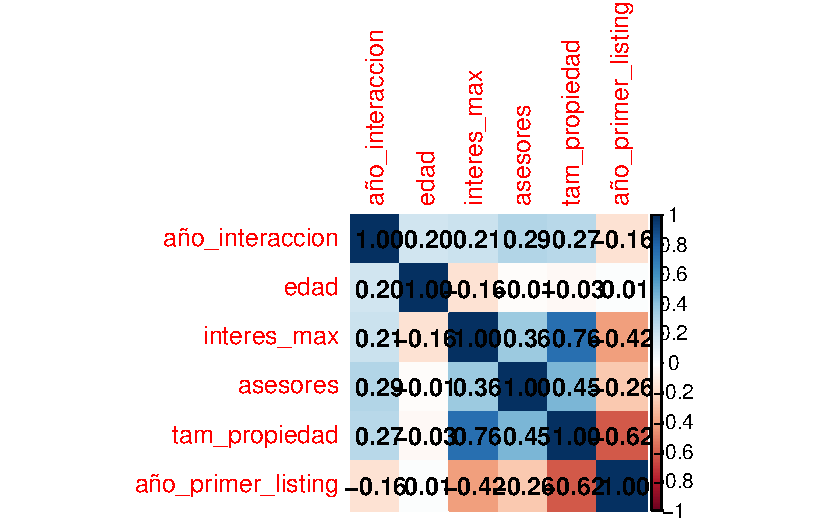
\includegraphics[keepaspectratio]{Inferencia_Bien_files/figure-pdf/unnamed-chunk-7-1.pdf}}

\begin{verbatim}
# A tibble: 6 x 19
  campaña  cliente_id propiedad año_interaccion ciclo_mercado sexo   edad origen
  <chr>    <fct>      <fct>               <dbl> <fct>         <fct> <dbl> <fct> 
1 AMAD811~ AMAD81101~ Ama Dabl~            1981 Spring        M        28 Spain 
2 AMAD811~ AMAD81101~ Ama Dabl~            1981 Spring        M        27 Spain 
3 AMAD811~ AMAD81101~ Ama Dabl~            1981 Spring        M        35 Spain 
4 AMAD811~ AMAD81101~ Ama Dabl~            1981 Spring        M        37 Spain 
5 AMAD811~ AMAD81101~ Ama Dabl~            1981 Spring        M        43 France
6 AMAD811~ AMAD81101~ Ama Dabl~            1981 Spring        M        38 Spain 
# i 11 more variables: rol_decision <fct>, partner_externo <lgl>,
#   interes_max <dbl>, compra <lgl>, decision_individual <lgl>, premium <lgl>,
#   lead_fallo <lgl>, friccion <lgl>, asesores <int>, tam_propiedad <dbl>,
#   año_primer_listing <dbl>
\end{verbatim}

Nueva Variable

Mide cuántos años pasaron desde que la propiedad fue listada por primera
vez hasta la interacción actual con el cliente. Refleja el tiempo de
exposición del activo inmobiliario, lo cual puede influir en la
probabilidad de compra:

Propiedades con mucha exposición pueden indicar sobreprecio, baja
demanda o problemas no observados.

Propiedades nuevas en el mercado suelen generar más interés y
conversiones rápidas.

También puede asociarse a estrategias de negocio como descuentos por
tiempo de publicación, rotación de inventario y urgencia comercial.

\begin{verbatim}
# A tibble: 6 x 20
  campaña  cliente_id propiedad año_interaccion ciclo_mercado sexo   edad origen
  <chr>    <fct>      <fct>               <dbl> <fct>         <fct> <dbl> <fct> 
1 AMAD811~ AMAD81101~ Ama Dabl~            1981 Spring        M        28 Spain 
2 AMAD811~ AMAD81101~ Ama Dabl~            1981 Spring        M        27 Spain 
3 AMAD811~ AMAD81101~ Ama Dabl~            1981 Spring        M        35 Spain 
4 AMAD811~ AMAD81101~ Ama Dabl~            1981 Spring        M        37 Spain 
5 AMAD811~ AMAD81101~ Ama Dabl~            1981 Spring        M        43 France
6 AMAD811~ AMAD81101~ Ama Dabl~            1981 Spring        M        38 Spain 
# i 12 more variables: rol_decision <fct>, partner_externo <lgl>,
#   interes_max <dbl>, compra <lgl>, decision_individual <lgl>, premium <lgl>,
#   lead_fallo <lgl>, friccion <lgl>, asesores <int>, tam_propiedad <dbl>,
#   año_primer_listing <dbl>, antiguedad_años <dbl>
\end{verbatim}

\pandocbounded{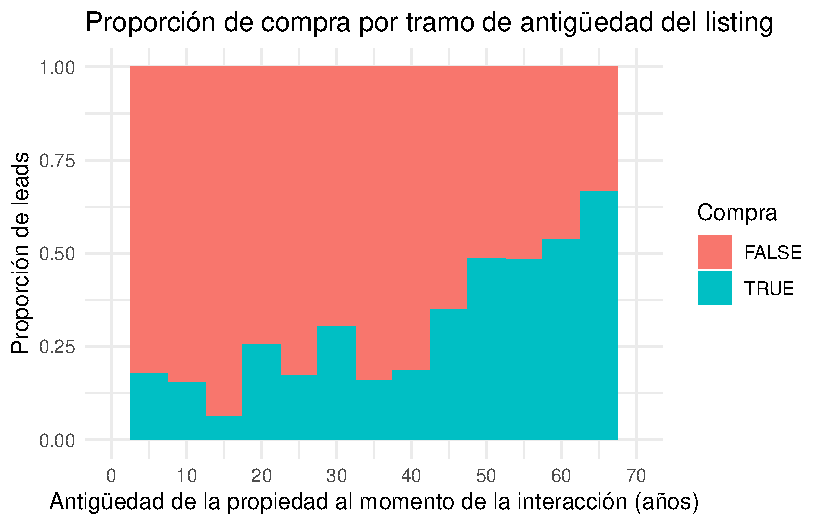
\includegraphics[keepaspectratio]{Inferencia_Bien_files/figure-pdf/unnamed-chunk-9-1.pdf}}

\pandocbounded{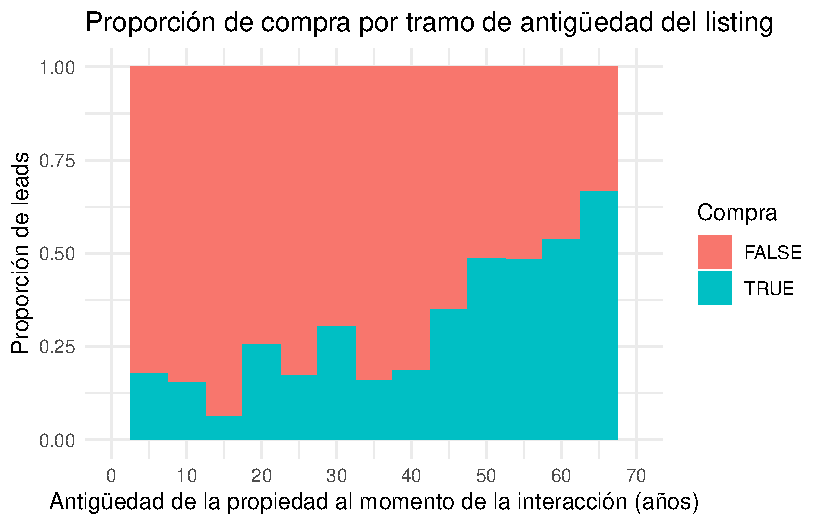
\includegraphics[keepaspectratio]{Inferencia_Bien_files/figure-pdf/unnamed-chunk-10-1.pdf}}

\pandocbounded{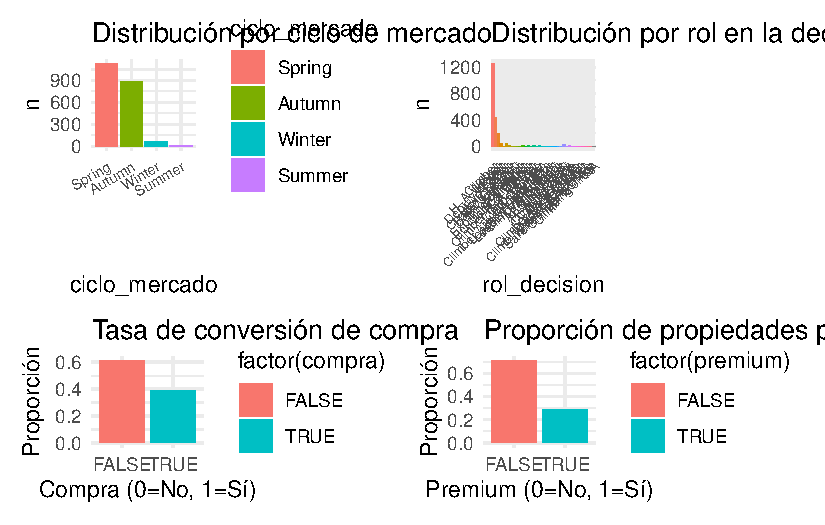
\includegraphics[keepaspectratio]{Inferencia_Bien_files/figure-pdf/unnamed-chunk-11-1.pdf}}

\pandocbounded{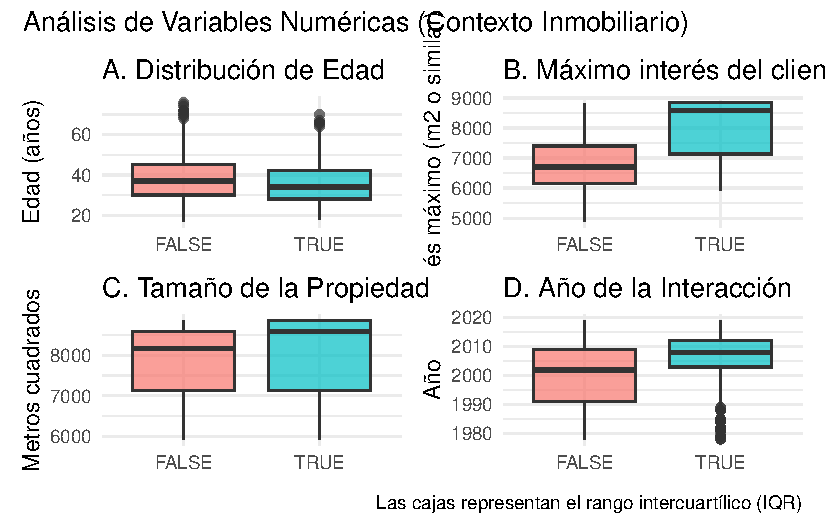
\includegraphics[keepaspectratio]{Inferencia_Bien_files/figure-pdf/unnamed-chunk-12-1.pdf}}

\pandocbounded{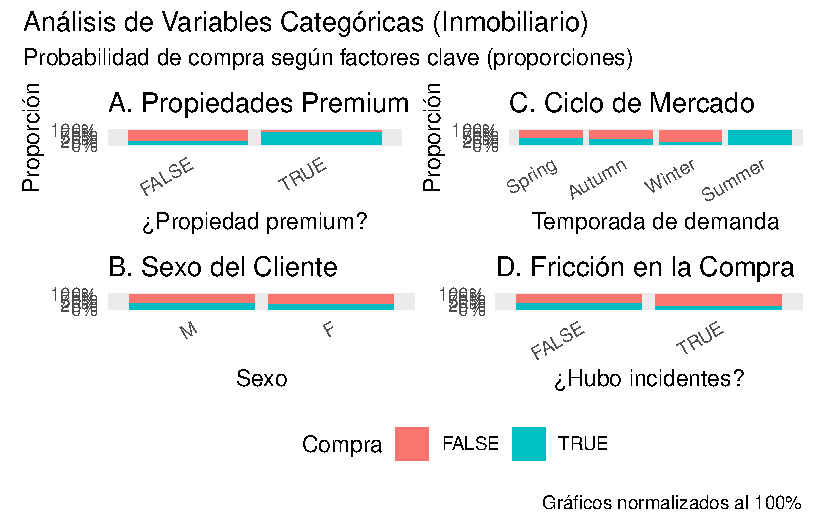
\includegraphics[keepaspectratio]{Inferencia_Bien_files/figure-pdf/unnamed-chunk-13-1.pdf}}

gráfico barras apiladas por proporción. sexo y éxito. se observa que la
proporción de éxito de hombre es apenas mayor, sin embargo, al tener tan
pocas observaciones sobre mujeres escaladoras, se considera que no hay
una relación fuerte como para definir sexo como predictora.

\section{Definicion de los modelos}\label{definicion-de-los-modelos}

USAMOS MODELO DE REGRESION LOGISTICA: nuestra variable de respuesta
``Y'' es binaria. En este caso es 1 si hubo succes (si la persona llego
a la cima de la montana), y 0 si hubo fracaso. Este tipo de regresión es
no lineal

\[\begin{aligned}
Y_i & \sim \text{Bern}(\pi_i) \\
\log\left(\frac{\pi_i}{1-\pi_i}\right) & = \beta_0 + \beta_1 X_1 + \beta_2 X_2
\end{aligned}\]

\(Y_i \sim \text{Bern}(\pi_i)\) (aleatoria): tener succes con
probabilidad de éxito \(\pi\).

\(\log(\frac{\pi}{1-\pi})\): es la transformación ``log odds'' que
hacemos para poder expresar nuestras probabilidades. nuestro modelo de
regresión lineal original nos da resultados en todo el mundo de los
reales. sin embargo, cuando trabajamos con variables binarias, nuestro
espacio de soluciones pasa a ser entre 0 y 1. tenemos que ajustar esto
para poder trabajar nuevamente con los reales, por eso aplicamos la
transformación. primero pasamos de ``probabilidad'' (pi) a ``odds'' o
``chances'', haciendo pi/(1-pi). lo que queremos calcular es cuantas
veces mas probable es ganar que perder. por ejemplo, si pi=0.5 entonces
odds va a ser 1, lo que quiere decir que con probabilidad 50\%, la
chance de ganar es una vez mas probable que perder. finalmente, le
aplicamos logaritmo a las odds, para que nuestro dominio sea todos los
reales. por ejemplo, en el caso de oods=1, al aplicar logaritmo
obtenemos 0, pero si nuestras odds fueran muy altas, el logaritmo seria
un numero positivo grande, y si las odds fueran muy bajas, el logaritmo
devuelve un numero negativo.

\(\beta_0\) (intercepto): probabilidad de éxito cuando todas las
variables \(X\) valen 0. ``probabilidad base''.

\(\beta_1\) (pendiente): cuanto aumenta (o disminuye) la probabilidad de
éxito si aumentamos \(X_1\) en una unidad. Si \(\beta > 0\): Aumenta la
probabilidad de exito. Si \(\beta < 0\): Disminuye la probabilidad.

MODELO DE REGRESION LOGISTICA JERARQUICO

POOLING: si los grupos comparten info entre si

ahora los datos tienen ``estructura''. Los escaladores pertenecen a
grupos (por ejemplo expedicion o monatana).

complete pooling: Ignora la montana. Asume que todas son iguales. (se
comparte toda la info)

No Pooling: Trata cada montana de forma independiente. (no se comparte
nada de la info)

Jerárquico (Partial Pooling): cada montana es unica (\(\beta_{0j}\)),
pero que todas pertenecen a una ``familia de montanas''. Las montanas
con pocos datos ``toman datos'' del promedio global. (se comparte algo
de info)

\[\begin{aligned}
\text{Nivel 1 (Datos):} \quad \log\left(\frac{\pi_{ij}}{1-\pi_{ij}}\right) & = \beta_{0j} + \beta_1 X_{ij1} \\
\text{Nivel 2 (Grupos):} \quad \beta_{0j} & \sim N(\beta_0, \sigma^2)
\end{aligned}\]

\(\beta_{0j}\) (efecto aleatorio/intercepto variando): Cada grupo \(j\)
(ej. cada montana o expedicion) tiene su propio ``punto de partida''.
\(\beta_0\) (Efecto fijo/Hiperparametro de media): Es el promedio global
de todas las montanas. \(\sigma\) (desviacion del grupo): Mide que tan
diferentes son las montanas entre si. Si \(\sigma\) es bajo: Todas las
montanas se parecen mucho (alto pooling). Si \(\sigma\) es alto: Las
montanas son muy distintas entre si (pooling bajo).

OBS: DEFINIMOS PRIORIS POCO INFORMATIVAS por que? Normal (0,2.5):
queremos evitar hacer overfitting cuando tenemos pocos datos (en nuestro
caso ``limpiamos'' mucho nuestra base de datos original) en la escala
logística, coeficientes mayores a 5 implican certeza prácticamente.
nosotros nos queremos posicionar ``en el medio'' y dejar que los datos
nos digan que paso. por otro lado, centramos en cero ya que queremos
tener una postura neutral. asumimos a priori que las variables no tienen
efecto sobre el éxito (por eso esta es 0). nuevamente dejamos que los
datos nos muestren que pasa. exp(1): varianza no puede ser negativa,
solo trabajamos con valores positivos.

\subsection{Modelo 1:}\label{modelo-1}

Definiremos el modelo 1 como el modelo con complete pooling con los
siguientes predictores: oxigeno, season, y year\_since\_first\_ascent.
Es decir, asumimos que todos los escaladores distribuyen de igual
manera.

OBS: no incluimos peak ya que no nos importa en que montaña estamos,
tratamos a todas por igual. Si incluimos peak estamos diferenciando a
las montañas. (``ignoramos los grupos y metemos a todos en la misma
bolsa'').

OBS: este modelo es nuestro punto de partida

De esta manera:

\[\boxed{
\hspace{0.5em}
\begin{aligned}
Y_{i} | \beta_{0}, \beta_1, \beta_2, \beta_3 & \sim \text{Bern}(\pi_{i}) && \text{(verosimilitud)} \\
\text{donde} \quad \log\left(\frac{\pi_{i}}{1-\pi_{i}}\right) & = \beta_{0} + \beta_1 X_{i1} + \beta_2 X_{i2} + \beta_3 X_{i3} \\
\beta_{0} & \sim N(0, 2.5^2) && \text{(intercepto global)} \\
\beta_1, \beta_2, \beta_3 & \overset{ind}{\sim} N(0, 2.5^2) && \text{(coeficientes fijos)}
\end{aligned}
\hspace{0.5em}
}\]

beta1, beta2 y beta 3 son nuestras predictoras (fijas)

variables:

\(Y_i\): Éxito del escalador \(i\). \(X_{i1}\): Uso de oxígeno.
\(X_{i2}\): Estación del año. \(X_{i3}\): Años desde el primer ascenso.

\subsection{Modelo 2:}\label{modelo-2}

Partial pooling por \textbf{expedicion}. Agregamos jerarquía en la
expedición j, tal como el libro.

\[
\boxed{
\hspace{0.5em}
\begin{aligned}
Y_{ij} | \beta_{0j}, \beta_1, \beta_2, \beta_3 & \sim \text{Bern}(\pi_{ij}) && \text{(verosimilitud)} \\
\text{with} \quad \log\left(\frac{\pi_{ij}}{1-\pi_{ij}}\right) & = \beta_{0j} + \beta_1 X_{ij1} + \beta_2 X_{ij2} + \beta_3 X_{ij3}\\
\beta_{0j} | \beta_{0c}, \sigma_{exp} & \overset{ind}{\sim} N(\beta_{0c}, \sigma_{exp}^2) && \text{(variabilidad entre expediciones)} \\
\beta_{0c} & \sim N(0, 2.5^2) && \text{(intercepto global)} \\
\beta_1, \beta_2, \beta_3 & \overset{ind}{\sim} N(0, 2.5^2) && \text{(coeficientes fijos)} \\
\sigma_{exp} & \sim \text{Exp}(1) && \text{(desvío est. entre expediciones)}
\end{aligned}
\hspace{0.5em}
}
\]

beta0, beta1 ,beta2 y beta3 son nuestras predictoras (fijas)

variables:

\(Y_i,j\): Éxito del escalador i en la expedición j. \(X_{i,j,1}\): Uso
de oxígeno. \(X_{i,j,2}\): Estación del año. \(X_{i,j,3}\): Años desde
el primer ascenso.

\subsection{Modelo 3}\label{modelo-3}

Partial Pooling por \textbf{peak} (agregamos jerarquía pico en vez de
escalación, para mostrar lo que a priori es un mal modelo o mal
conceptualmente hablando agrupar por pico ). Hay individuos dentro del
mismo grupo muy divergentes entre si.

\[\boxed{
\hspace{0.5em}
\begin{aligned}
Y_{ik} | \beta_{0k}, \beta_1, \beta_2, \beta_3 & \sim \text{Bern}(\pi_{ik}) && \text{(verosimilitud)} \\
\text{with} \quad \log\left(\frac{\pi_{ik}}{1-\pi_{ik}}\right) & = \beta_{0k} + \beta_1 X_{ik1} + \beta_2 X_{ik2} + \beta_3 X_{ik3} \\
\beta_{0k} | \beta_{0c}, \sigma_{peak} & \overset{ind}{\sim} N(\beta_{0c}, \sigma_{peak}^2) && \text{(variabilidad entre picos)} \\
\beta_{0c} & \sim N(0, 2.5^2) && \text{(intercepto global)} \\
\beta_1, \beta_2, \beta_3 & \overset{ind}{\sim} N(0, 2.5^2) && \text{(coeficientes fijos)} \\
\sigma_{peak} & \sim \text{Exp}(1) && \text{(desvío est. entre picos)}
\end{aligned}
\hspace{0.5em}
}\]

beta1, beta2 y beta3 son nuestras predictoras

variables

\(Y_i,k\): Éxito del escalador i en peak k. \(X_{i,k,1}\): Uso de
oxígeno. \(X_{i,k,2}\): Estación del año. \(X_{i,k,3}\): Años desde el
primer ascenso.

\subsubsection{Modelo 4}\label{modelo-4}

Jerarquía con Season.

\[\boxed{
\hspace{0.5em}
\begin{aligned}
Y_{is} | \beta_{0s}, \beta_1, \beta_2, \beta_3 & \sim \text{Bern}(\pi_{is}) && \text{(verosimilitud)} \\
\text{with} \quad \log\left(\frac{\pi_{is}}{1-\pi_{is}}\right) & = \beta_{0s} + \beta_1 X_{is1} + \beta_2 X_{is2} + \beta_3 X_{is3} \\
\beta_{0s} | \beta_{0c}, \sigma_{peak} & \overset{ind}{\sim} N(\beta_{0c}, \sigma_{peak}^2) && \text{(variabilidad entre picos)} \\
\beta_{0c} & \sim N(0, 2.5^2) && \text{(intercepto global)} \\
\beta_1, \beta_2, \beta_3 & \overset{ind}{\sim} N(0, 2.5^2) && \text{(coeficientes fijos)} \\
\sigma_{peak} & \sim \text{Exp}(1) && \text{(desvío est. entre picos)}
\end{aligned}
\hspace{0.5em}
}\]

beta1, beta2 y beta3 son nuestras predictoras

variables

\(Y_i,s\): Éxito del escalador i en season s. \(X_{i,s,1}\): Uso de
oxígeno. \(X_{i,s,2}\): Estación del año. \(X_{i,s,3}\): Años desde el
primer ascenso.

\begin{verbatim}
# A tibble: 6 x 21
  campaña  cliente_id propiedad año_interaccion ciclo_mercado sexo   edad origen
  <chr>    <fct>      <fct>               <dbl> <fct>         <fct> <dbl> <fct> 
1 AMAD811~ AMAD81101~ Ama Dabl~            1981 Spring        M        28 Spain 
2 AMAD811~ AMAD81101~ Ama Dabl~            1981 Spring        M        27 Spain 
3 AMAD811~ AMAD81101~ Ama Dabl~            1981 Spring        M        35 Spain 
4 AMAD811~ AMAD81101~ Ama Dabl~            1981 Spring        M        37 Spain 
5 AMAD811~ AMAD81101~ Ama Dabl~            1981 Spring        M        43 France
6 AMAD811~ AMAD81101~ Ama Dabl~            1981 Spring        M        38 Spain 
# i 13 more variables: rol_decision <fct>, partner_externo <lgl>,
#   interes_max <dbl>, compra <lgl>, decision_individual <lgl>, premium <lgl>,
#   lead_fallo <lgl>, friccion <lgl>, asesores <int>, tam_propiedad <dbl>,
#   año_primer_listing <dbl>, antiguedad_años <dbl>, tramo_antiguedad <fct>
\end{verbatim}

\section{Corrida de los modelos}\label{corrida-de-los-modelos}

\subsection{Modelos}\label{modelos}

\section{Modelo 1}\label{modelo-1-1}

\pandocbounded{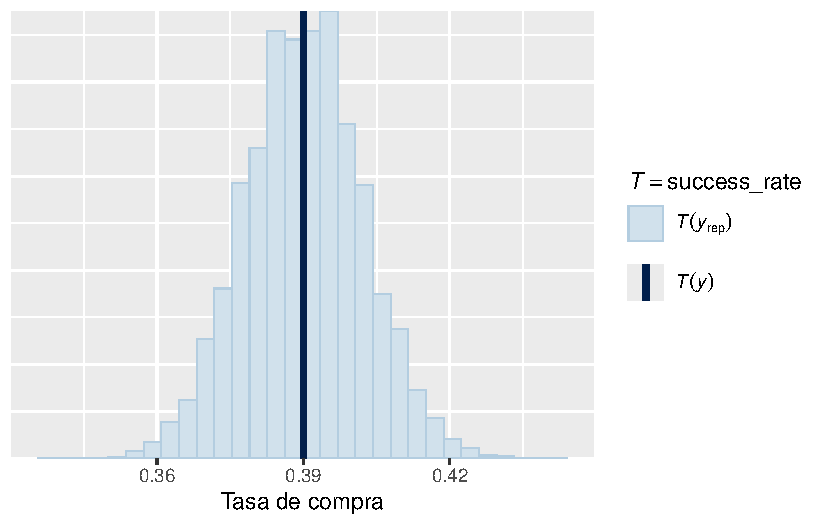
\includegraphics[keepaspectratio]{Inferencia_Bien_files/figure-pdf/unnamed-chunk-16-1.pdf}}

La barra vertical es el éxito promedio del dataframe. El resto en
celeste es la tasa de éxito en nuestros 100 dataframes simulados.

Modelo 2

\pandocbounded{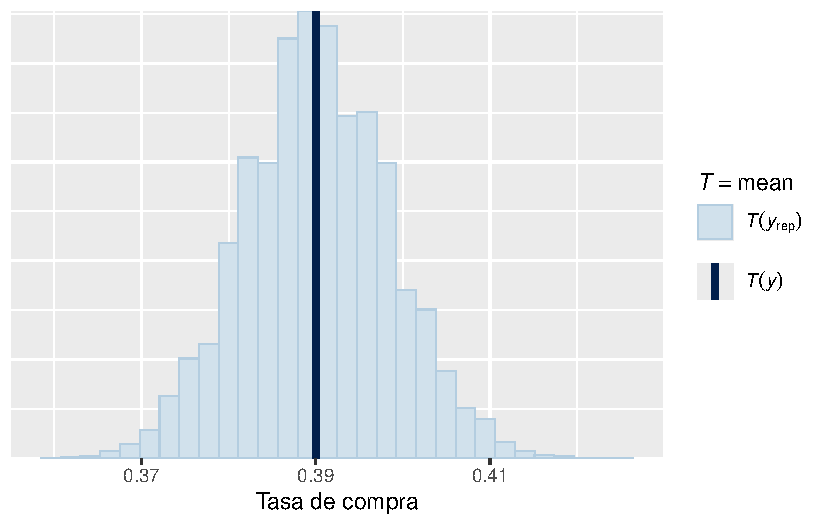
\includegraphics[keepaspectratio]{Inferencia_Bien_files/figure-pdf/unnamed-chunk-17-1.pdf}}

Notamos que este modelo tiene una mejoría respecto al anterior, pero de
igual forma pensamos que todavía se puede mejorar más

Modelo 3

\pandocbounded{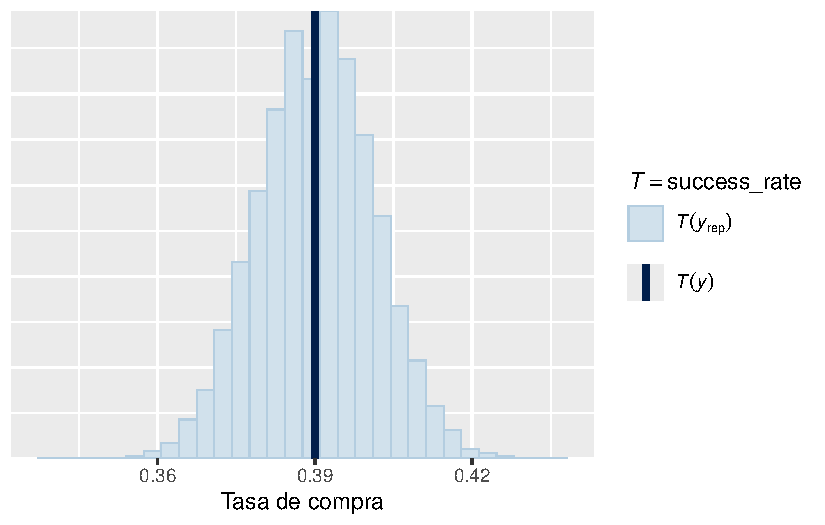
\includegraphics[keepaspectratio]{Inferencia_Bien_files/figure-pdf/unnamed-chunk-18-1.pdf}}

\section{Modelo 4}\label{modelo-4-1}

\pandocbounded{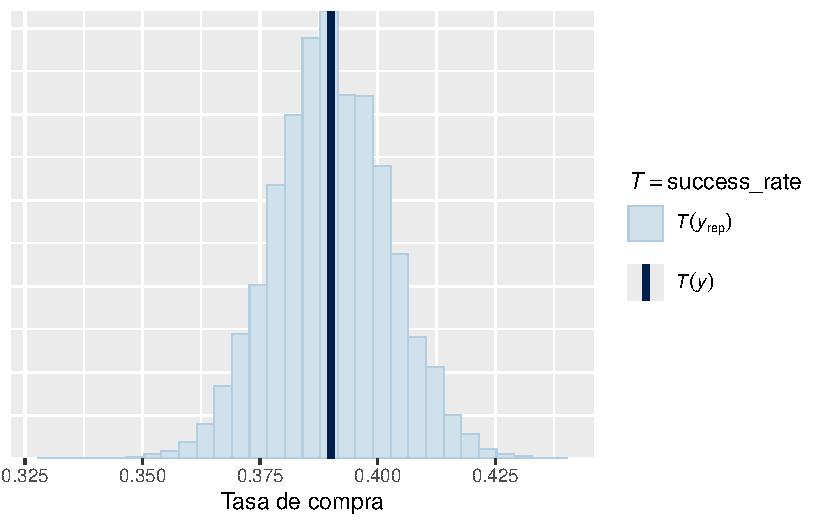
\includegraphics[keepaspectratio]{Inferencia_Bien_files/figure-pdf/unnamed-chunk-19-1.pdf}}

\pandocbounded{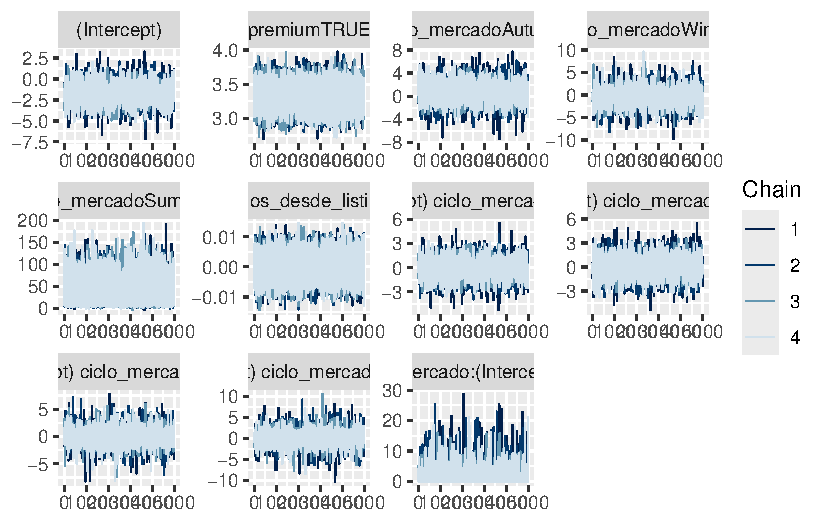
\includegraphics[keepaspectratio]{Inferencia_Bien_files/figure-pdf/unnamed-chunk-19-2.pdf}}

\section{PP\_Checks:}\label{pp_checks}

\pandocbounded{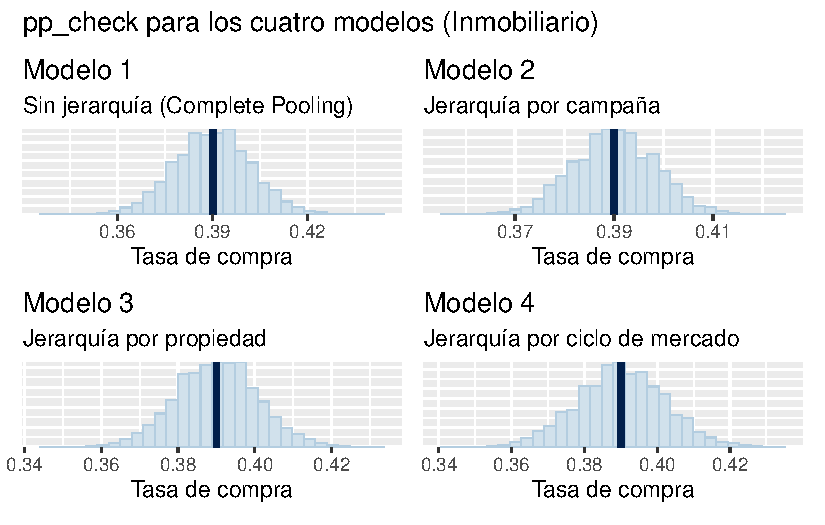
\includegraphics[keepaspectratio]{Inferencia_Bien_files/figure-pdf/unnamed-chunk-20-1.pdf}}

Se observa de forma visual que no existen diferencias sustanciales entre
los modelos. Se podría decir que en principio no aporta una mejoría
realizar agrupamiento.

\section{MCMC diagnostics}\label{mcmc-diagnostics}

\begin{verbatim}
Priors for model 'modjs' 
------
Intercept (after predictors centered)
 ~ normal(location = 0, scale = 2.5)

Coefficients
  Specified prior:
    ~ normal(location = [0,0,0,...], scale = [2.5,2.5,2.5,...])
  Adjusted prior:
    ~ normal(location = [0,0,0,...], scale = [ 5.51, 5.05,15.14,...])

Covariance
 ~ decov(reg. = 1, conc. = 1, shape = 1, scale = 1)
------
See help('prior_summary.stanreg') for more details
\end{verbatim}

\pandocbounded{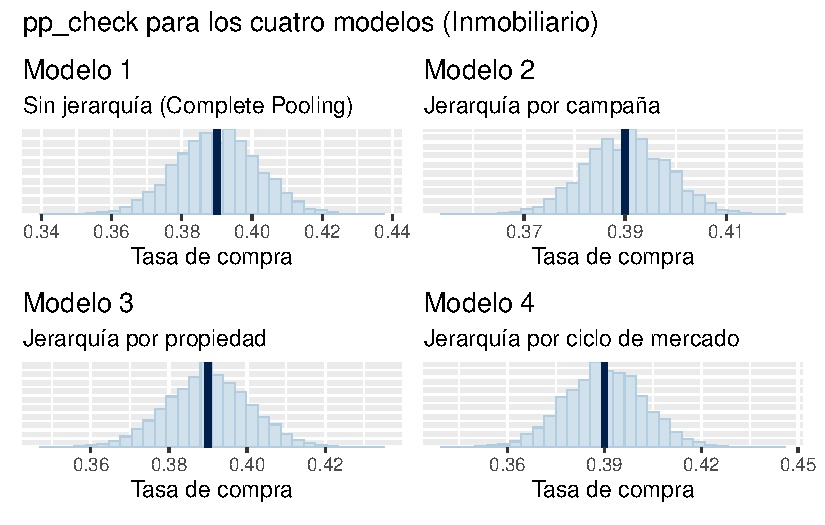
\includegraphics[keepaspectratio]{Inferencia_Bien_files/figure-pdf/unnamed-chunk-21-1.pdf}}

\pandocbounded{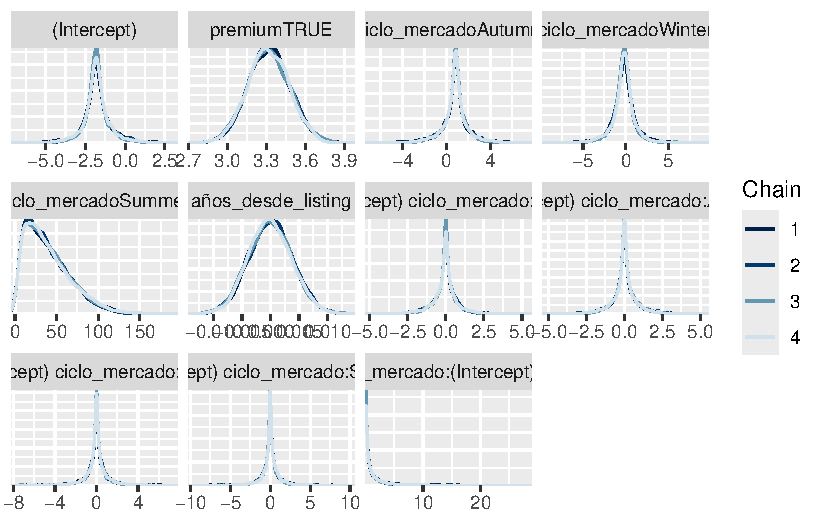
\includegraphics[keepaspectratio]{Inferencia_Bien_files/figure-pdf/unnamed-chunk-21-2.pdf}}

\pandocbounded{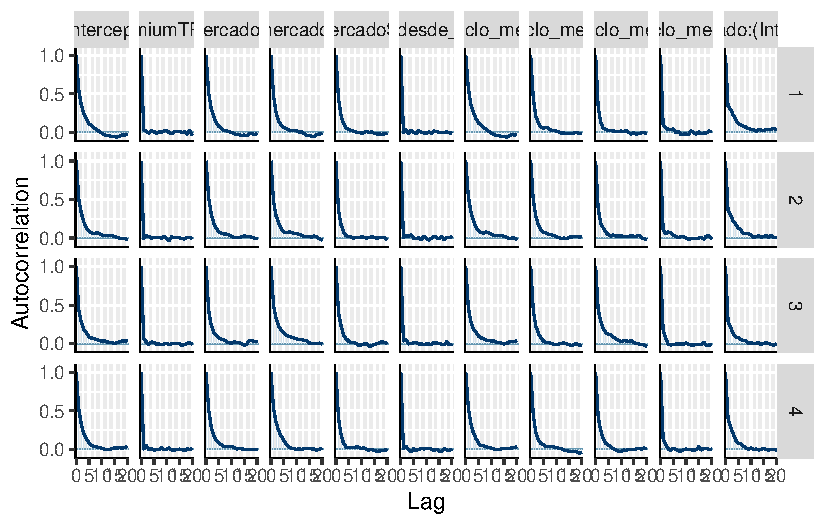
\includegraphics[keepaspectratio]{Inferencia_Bien_files/figure-pdf/unnamed-chunk-21-3.pdf}}

\begin{verbatim}
                                 (Intercept) 
                                     0.24870 
                                 premiumTRUE 
                                     0.87620 
                         ciclo_mercadoAutumn 
                                     0.26945 
                         ciclo_mercadoWinter 
                                     0.24635 
                         ciclo_mercadoSummer 
                                     0.37660 
                          años_desde_listing 
                                     0.88870 
         b[(Intercept) ciclo_mercado:Spring] 
                                     0.23825 
         b[(Intercept) ciclo_mercado:Autumn] 
                                     0.30675 
         b[(Intercept) ciclo_mercado:Winter] 
                                     0.32580 
         b[(Intercept) ciclo_mercado:Summer] 
                                     0.65680 
Sigma[ciclo_mercado:(Intercept),(Intercept)] 
                                     0.21905 
\end{verbatim}

\begin{verbatim}

Model Info:
 function:     stan_glmer
 family:       binomial [logit]
 formula:      compra ~ premium + ciclo_mercado + años_desde_listing + (1 | 
       ciclo_mercado)
 algorithm:    sampling
 sample:       20000 (posterior sample size)
 priors:       see help('prior_summary')
 observations: 2069
 groups:       ciclo_mercado (4)

Estimates:
                                               mean   sd   10%   50%   90%
(Intercept)                                  -1.8    0.9 -2.7  -1.8  -0.8 
premiumTRUE                                   3.3    0.2  3.1   3.3   3.5 
ciclo_mercadoAutumn                           0.8    1.2 -0.6   0.8   2.0 
ciclo_mercadoWinter                          -0.3    1.4 -1.7  -0.2   1.2 
ciclo_mercadoSummer                          39.8   27.4  9.6  34.1  78.4 
años_desde_listing                            0.0    0.0  0.0   0.0   0.0 
b[(Intercept) ciclo_mercado:Spring]          -0.1    0.8 -1.0   0.0   0.8 
b[(Intercept) ciclo_mercado:Autumn]           0.0    0.9 -0.9   0.0   0.9 
b[(Intercept) ciclo_mercado:Winter]           0.0    1.0 -1.0   0.0   1.0 
b[(Intercept) ciclo_mercado:Summer]           0.0    1.1 -1.0   0.0   1.0 
Sigma[ciclo_mercado:(Intercept),(Intercept)]  1.1    2.1  0.0   0.3   3.0 

Fit Diagnostics:
           mean   sd   10%   50%   90%
mean_PPD 0.4    0.0  0.4   0.4   0.4  

The mean_ppd is the sample average posterior predictive distribution of the outcome variable (for details see help('summary.stanreg')).

MCMC diagnostics
                                             mcse Rhat n_eff
(Intercept)                                  0.0  1.0   4974
premiumTRUE                                  0.0  1.0  17524
ciclo_mercadoAutumn                          0.0  1.0   5389
ciclo_mercadoWinter                          0.0  1.0   4927
ciclo_mercadoSummer                          0.3  1.0   7532
años_desde_listing                           0.0  1.0  17774
b[(Intercept) ciclo_mercado:Spring]          0.0  1.0   4765
b[(Intercept) ciclo_mercado:Autumn]          0.0  1.0   6135
b[(Intercept) ciclo_mercado:Winter]          0.0  1.0   6516
b[(Intercept) ciclo_mercado:Summer]          0.0  1.0  13136
Sigma[ciclo_mercado:(Intercept),(Intercept)] 0.0  1.0   4381
mean_PPD                                     0.0  1.0  20328
log-posterior                                0.0  1.0   7794

For each parameter, mcse is Monte Carlo standard error, n_eff is a crude measure of effective sample size, and Rhat is the potential scale reduction factor on split chains (at convergence Rhat=1).
\end{verbatim}

\begin{verbatim}
# A tibble: 6 x 5
  term                    estimate std.error conf.low conf.high
  <chr>                      <dbl>     <dbl>    <dbl>     <dbl>
1 (Intercept)             -3.99       0.918   -5.86     -2.25  
2 seasonAutumn             1.73       0.619    0.533     2.94  
3 seasonWinter            -0.106      1.74    -3.71      3.25  
4 seasonSummer            35.8       26.6      5.83    110.    
5 year_since_first_ascent -0.00106    0.0177  -0.0354    0.0347
6 oxygen_usedTRUE          6.15       0.522    5.20      7.25  
\end{verbatim}

\begin{longtable}[t]{lrrrr}
\caption{\label{tab:unnamed-chunk-23}Estimación de efectos fijos con interpretación de impacto en retención de clientes}\\
\toprule
term & estimate & std.error & conf.low & conf.high\\
\midrule
Intercepto & -3.987 & 0.918 & -5.858 & -2.253\\
ciclo\_mercadoAutumn & 1.726 & 0.619 & 0.533 & 2.940\\
ciclo\_mercadoWinter & -0.106 & 1.739 & -3.706 & 3.246\\
ciclo\_mercadoSummer & 35.814 & 26.553 & 5.827 & 110.084\\
antiguedad\_años & -0.001 & 0.018 & -0.035 & 0.035\\
\addlinespace
premium & 6.146 & 0.522 & 5.204 & 7.246\\
\bottomrule
\end{longtable}

\pandocbounded{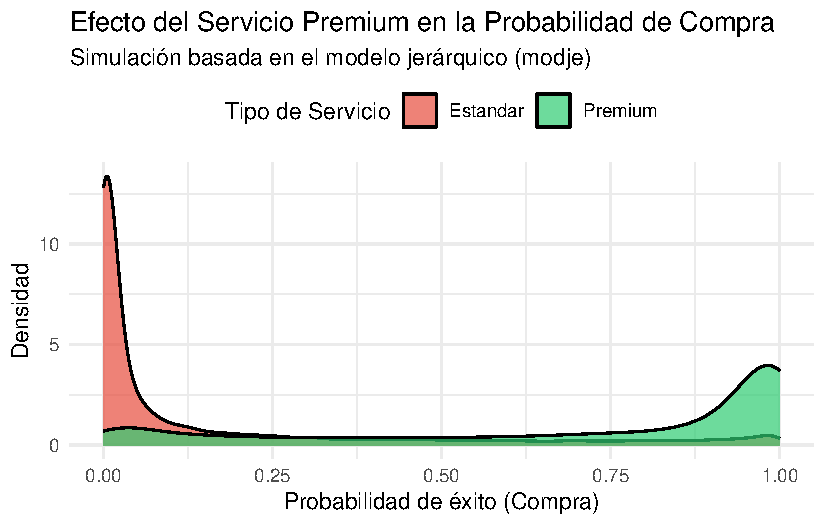
\includegraphics[keepaspectratio]{Inferencia_Bien_files/figure-pdf/unnamed-chunk-24-1.pdf}}

\pandocbounded{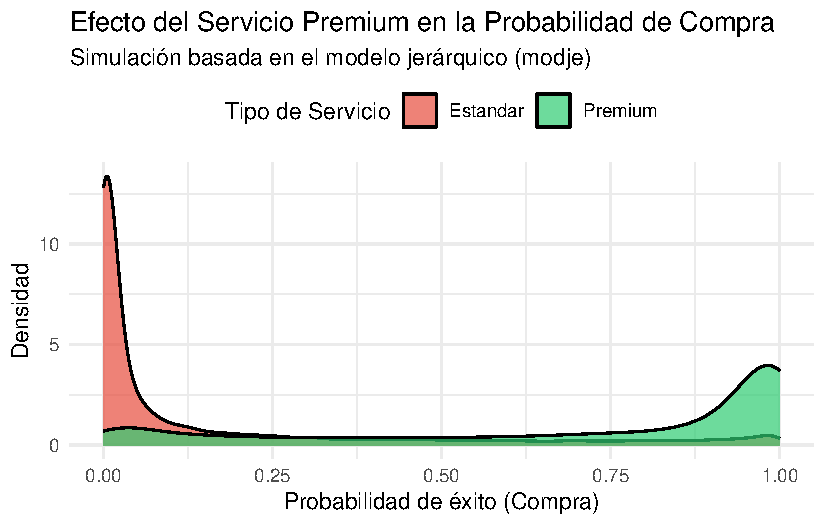
\includegraphics[keepaspectratio]{Inferencia_Bien_files/figure-pdf/unnamed-chunk-25-1.pdf}}

\pandocbounded{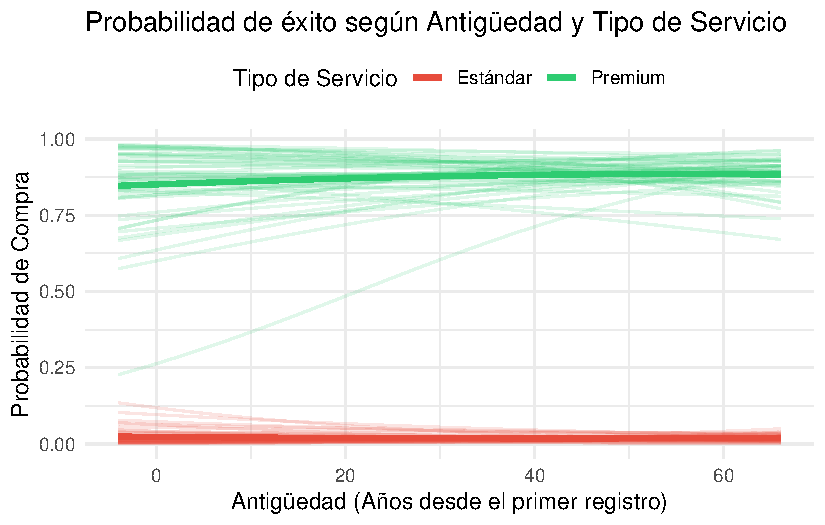
\includegraphics[keepaspectratio]{Inferencia_Bien_files/figure-pdf/unnamed-chunk-26-1.pdf}}

Modelo sin oxigeno

\begin{longtable}[t]{lrrrr}
\caption{\label{tab:unnamed-chunk-28}Estimación de efectos fijos para modelo sin oxígeno}\\
\toprule
term & estimate & std.error & conf.low & conf.high\\
\midrule
(Intercept) & -3.6085705 & 0.8683727 & -4.7851841 & -2.5462811\\
seasonAutumn & -0.0720445 & 0.5732634 & -0.8217776 & 0.6611852\\
seasonWinter & -1.1419446 & 1.7162429 & -3.4014098 & 1.0027344\\
seasonSummer & 33.6362966 & 27.6343194 & 8.4793551 & 79.5369982\\
year\_since\_first\_ascent & 0.0491697 & 0.0166085 & 0.0286509 & 0.0716704\\
\bottomrule
\end{longtable}




\end{document}
